\chapter{SISOTool-Designed Controller Response} \label{app:sisoToolDControllerTest}
\textbf{Name: Group 630}\\
\textbf{Date: 15/04 - 2016}

\subsubsection{Purpose}
Checking the stability of the controller designed from Matlab's SISOTool upon basic stimulation.

\subsubsection{Setup}
The Cubli is put in an unstable equilibrium at approximately \SI{0}{^{\circ}}. 
It is plugged to a computer from which the correct code can be sent, started and to which the data can later be retrieved, through USB over an Secure SHell (SSH) connection.

\subsubsection{List of Equipment}
\begin{table}[H]
\begin{tabular}{|p{8cm}|p{2cm}|p{4cm}|}
\hline%------------------------------------------------------------------------------------
  \textbf{Instrument}    &  \textbf{AAU-no.}          &  \textbf{Type} \\
\hline%------------------------------------------------------------------------------------
  Computer               &            &  Asus UX301LA  \\
\hline%------------------------------------------------------------------------------------
Dedicated Power Supply of Cubli \small{(24 V - 3 A)} &  AAU3                   &  XP Power, AEB70US24                 \\
\hline%------------------------------------------------------------------------------------------------------------
\end{tabular}
\end{table}

\subsubsection{Procedure}

\begin{enumerate}
  \item Plug the power supply given with the Cubli setup to a \si{220}{V} power outlet.
  \item Wait until the blue LEDs on the Beaglebone Black start blinking slowly and connect the USB cable to the PC.
  \item Send the binary compiled program of the controller to the board.
  \item Connect to a distant terminal on the Beaglebone Black through SSH and launch the program.
  \item Let the program run until the Cubli has fallen down. Give it a slight push if it still stands up and still.
  \item Stop the program (by pressing \textit{Q} and \textit{ENTER}).
  \item Retrieve the log file from the Cubli setup with the recorded data.
\end{enumerate}

\subsubsection{Results}

\begin{minipage}{0.45\linewidth}
	\begin{figure}[H]
		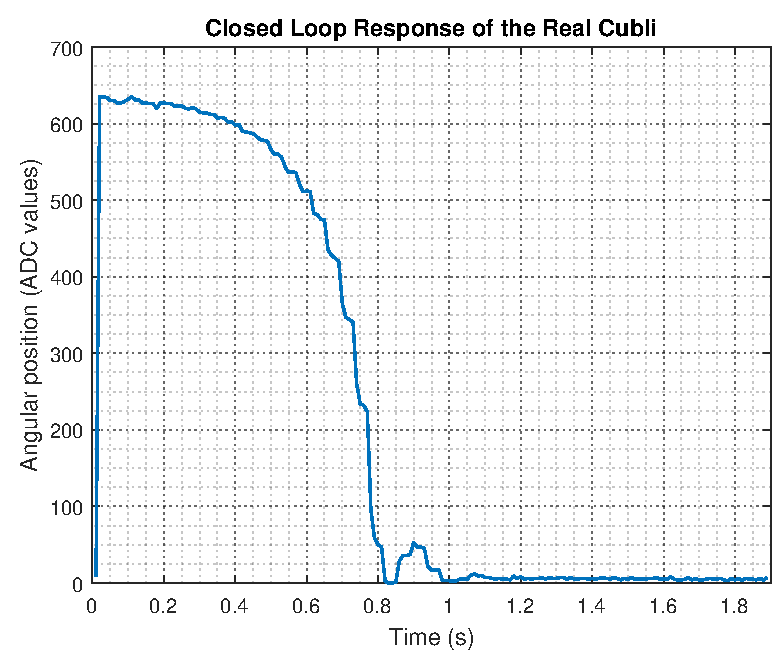
\includegraphics[scale=.53]{figures/ADCTestTustinPre}
		\captionsetup{justification=centering}
		\captionof{figure}{Raw values from the ADC}
		\label{ADCTestTustinPre}
	\end{figure}\vspace{-5mm}
\end{minipage}
\hspace{0.03\linewidth}
\begin{minipage}{0.45\linewidth}
	\begin{figure}[H]\vspace{-4mm}
		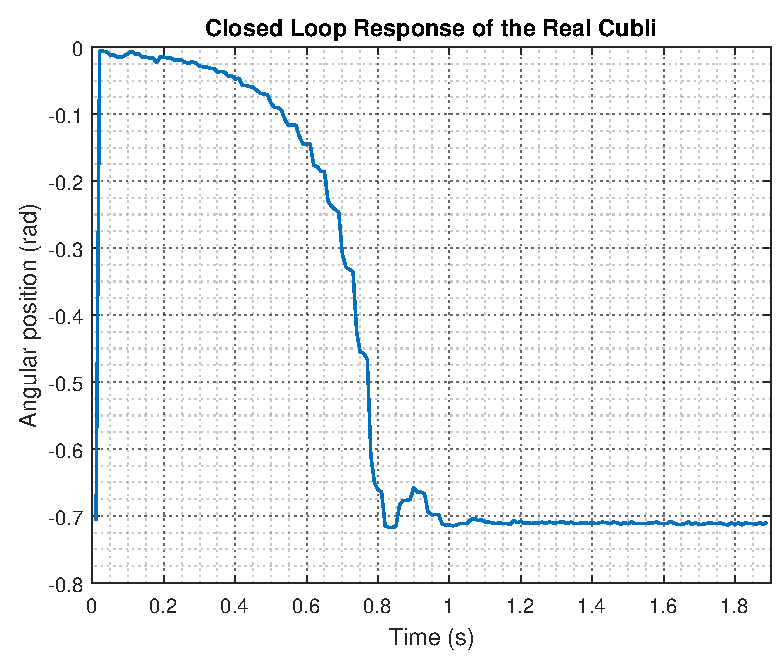
\includegraphics[scale=.53]{figures/positionTestTustinPre}
		\captionsetup{justification=centering}
		\captionof{figure}{Angular position of the Cubli}
		\label{positionTestTustinPre}
	\end{figure}\vspace{-5mm}
\end{minipage}
\\
\begin{minipage}{0.45\linewidth}
	\begin{figure}[H]
		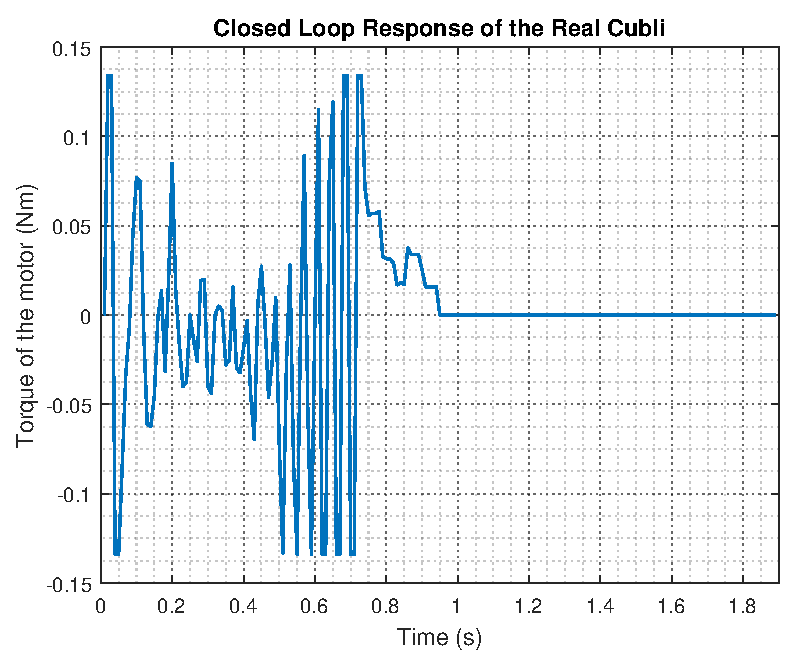
\includegraphics[scale=.53]{figures/torqueTestTustinPre}
		\captionsetup{justification=centering}
		\captionof{figure}{Torque values asked to the motor}
		\label{torqueTestTustinPre}
	\end{figure}\vspace{-5mm}
\end{minipage}
\hspace{0.03\linewidth}
\begin{minipage}{0.45\linewidth}
	\begin{figure}[H]\vspace{-4mm}
		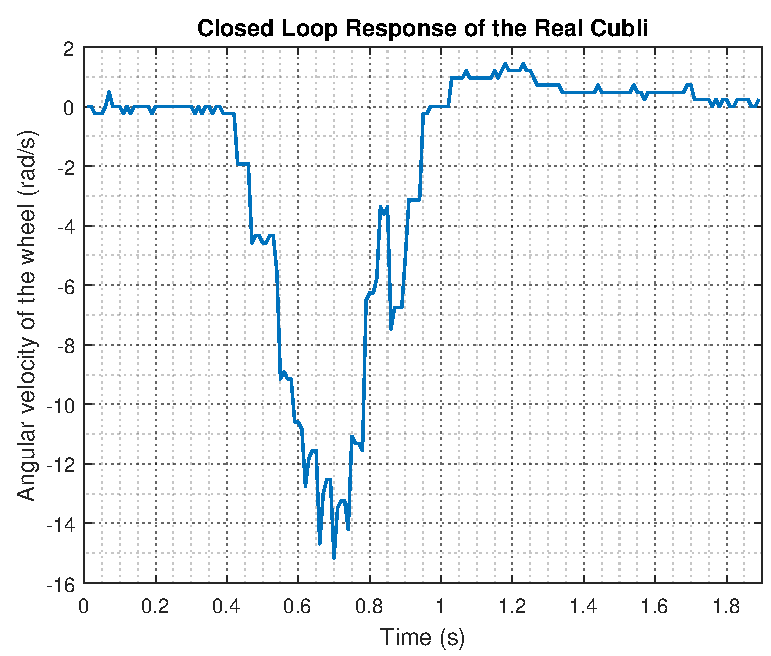
\includegraphics[scale=.53]{figures/wheelTestTustinPre}
		\captionsetup{justification=centering}
		\captionof{figure}{Angular velocity of the wheel}
		\label{wheelTestTustinPre}
	\end{figure}\vspace{-5mm}
\end{minipage}
